\section{Reverse Engineering}
Assembler als Haupt-Programmiersprache für Softwareprojekte hat auf Grund der großen Verbreitung einer Vielzahl von Hochsprachen, mit samt deren Vorteilen wie höheres Abstraktionsniveau, umfangreiche Werkzeuge, hohe Portierbarkeit und Wirtschaftlichkeit von Wartung und Kollaboration in Teams, stark an Bedeutung verloren. Auch sind die Hauptstärken von Assembler Schnelligkeit und geringe Codegröße durch das Aufkommen hochoptimierender Compiler und dem exponentiellem Wachstum von Prozessorleistung und Speicherkapazitäten in den Hintergrund getreten.

Doch auch ohne dass heute noch viel direkt in Assembler programmiert wird, ist die Kenntnis der Sprache unverzichtbar für das sogenannte \emph{Reverse Engineering}. Damit bezeichnet man im Software-Kontext die Disassemblierung und Analyse von binärem Programmcode, also allem übersetzten, ausführbaren Code eines Computers. Es lässt sich als ein ``Zurückgehen im Entwicklungsprozess'' beschreiben.\cite{Warden1992}

Dies kann aus vielerlei Motivation möglich sein:
\begin{itemize}
\item Debugging von Compilerfehlern oder Programmen ohne Quelltext,
\item Schadcode-Analyse z.B. in der Anti-Virus-Industrie,
\item Forensische Analyse nach einer Sicherheitskompromitierung (``Hacker-Angriff''),
\item Sicherheitslücken suchen und aufdecken durch Sicherheitsforscher,
\item Umgehung von Kopierschutz durch Entwickeln von \emph{Cracks} (binäre Patches),
\item Umgehung von Kopierschutz durch \emph{Keygeneratoren} – Analyse und Nachbau des Lizensierungsschemas einer kommerziellen Anwendung,
\item oder auch der Analyse, Umgehung oder Entfernung von \emph{Digital Rights Management}.
\end{itemize}

Die allgemeine Vorgehensweise soll am Beispiel der Schadcode-Analyse kurz beschrieben werden: ein Anti-Virus-Hersteller und unabhängiges Forscherteam enthält unbekannten Virencode durch Einsendung eines Tipgebers dem Einsammeln von infizierten Dateien auf speziellen ``Locksystemen'' (\emph{Honey-pots}). Dieser auch als \emph{Sample} bezeichnete Binärcode wird in einem Disassembler, wie \emph{IDA Pro, OllyDbg} oder dem \emph{GNU Debugger}\cite{disasm}, geladen und zunächst statisch analysiert. Neben dem Assembler-Listing und vorinitialisierten Daten wie Strings und Tabellen, erhält man oft auch Informationen zu Programmelementen höherer Abstraktionslevel wie Structs, Klassen und deren Methoden und Funktions- und Variablennamen (wenn sie zwecks Ausführens oder Debuggens erforderlich waren bzw. absichtlich in das Programm kompiliert wurden).
Oft lassen sich auch Flussdiagramme und Aktivierungsbäume der Funktionsaufrufe automatisch generieren.

\begin{figure}[h]
  \begin{center}
    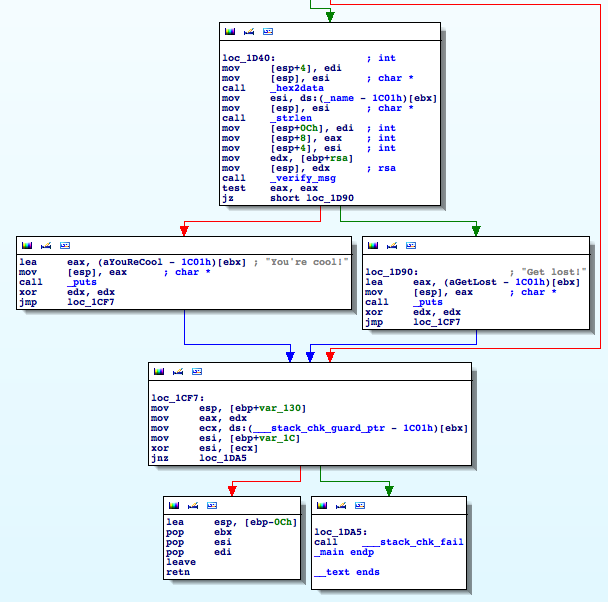
\includegraphics[width=0.85\textwidth]{IDA-pro-flowchart.png}
  \end{center}
  \caption{Flussdiagramm eines Programmsegments im IDA Pro Disassembler}
\end{figure}

Da diese Disassembler oft auch auf Seiten der Virenentwicklers zum Grundwerkzeug gehören, werden in der Praxis oft Verschleierungs- oder sogar Verschlüsselungstechniken eingesetzt, die statische Code-Analyse erschweren oder unmöglich machen. Die meisten Disassembler sind aber gleichzeitig auch Debugger und erlauben die Analyse zur Laufzeit – f\"ur Schadcode sinnvollerweise in einer geschützten Laborumgebung. Ein \emph{Trace} durch den Programmablauf hinterlässt dann eine Spur des tatsächlich ausgeführten, aktiven Codes und dem Zustand aller Register- und Speicherinhalte.

Das Umgehen von Software-Sicherungen als Kopier- oder Zugangsschutz ist ein Einsatzfeld von Reverse-Engineering-Techniken in einer legalen Grauzone. Die Verwertung  der Ergebnisse solcher Analysen bricht in der Regel geltendes Patent-, Eigentums- und/oder Urheberrecht. Es gibt jedoch auch Enthusiasten, die \emph{Cracking} aus ``sportlichen'' Gründen betreiben und von den facettenreichen Fähigkeiten fasziniert sind die dazu häufig nötig sind. Ein legaler Weg beschreiten sogenannte \emph{Crackmes}\cite{crackme}, kleine Programme die von anderen \emph{Reversern} geschrieben wurden um sich gegenseitig auszuprobieren oder herauszufordern.

Ein weiteres Feld in dem Assembler-Code geschrieben und gelesen werden muss, ist das Entwickeln bzw. Analysieren von \emph{Exploits}. So bezeichnet man kurze Programme zum aktiven Ausnutzen von Sicherheitslücken. Meist geht es dabei darum subversiv, eigenen Code in fremde Computersysteme einzuschleusen und sich nicht-autorisierten Zugang zu verschaffen. Assembler taucht hier meist in Form von \emph{Shellcode} auf. Code der so heißt, da er in der Regel zum Starten einer privilegierten, fernsteuerbaren Shell auf dem Fremdsystem eingeschleust wird. Der Shellcode wird in Form einer absichtlich falsch zusammengesetzten Dateneingabe eingebracht, auf die die entgegennehmende Software fehlerhaft reagiert. Der Shellcode befindet sich dann schon auf dem Stack oder Heap des anfälligen Programms und muss geschickt unter Ausnutzung der Sicherheitslücke angesprungen werden. Gute Assemblerkentnisse sind für den Exploit-Programmierer Voraussetzung. Die Motivationen sind wiederum vielschichtig und reichen von wissenschaftlichem Forschungsgeist, über persönlichen Ehrgeiz bis hin zu kriminellen Absichten.
